%%%%%%%%%%%%%%%%%%%%%%%%%%%%%%%%%%%%%%%%%
% baposter Portrait Poster
% LaTeX Template
% Version 1.0 (15/5/13)
%
% Created by:
% Brian Amberg (baposter@brian-amberg.de)
%
% This template has been downloaded from:
% http://www.LaTeXTemplates.com
%
% License:
% CC BY-NC-SA 3.0 (http://creativecommons.org/licenses/by-nc-sa/3.0/)
%
%%%%%%%%%%%%%%%%%%%%%%%%%%%%%%%%%%%%%%%%%

\documentclass[a0paper,portrait]{baposter}
\usepackage[utf8]{inputenc} % input encoding : utf8, latin9, latin1
\usepackage[french]{babel} % document language : typography + titles...
\usepackage[T1]{fontenc} % font encoding : ö = single letter and not o + accent
\usepackage{enumitem}

\usepackage{tikz}
\usetikzlibrary{shapes,arrows}
\fboxsep=0mm%padding thickness
\fboxrule=4pt%border thickness

\usepackage{graphicx}
%\usepackage{caption}


\usepackage[font=small,labelfont=bf]{caption} % Required for specifying captions to tables and figures
\usepackage{subcaption}
\usepackage{booktabs} % Horizontal rules in tables
\usepackage{relsize} % Used for making text smaller in some places

\graphicspath{{figures/}} % Directory in which figures are stored

\definecolor{bordercol}{RGB}{40,40,40} % Border color of content boxes
\definecolor{headercol1}{RGB}{186,215,230} % Background color for the header in the content boxes (left side)
\definecolor{headercol2}{RGB}{80,80,80} % Background color for the header in the content boxes (right side)
\definecolor{headerfontcol}{RGB}{0,0,0} % Text color for the header text in the content boxes
\definecolor{boxcolor}{RGB}{186,215,230} % Background color for the content in the content boxes

\begin{document}

\background{ % Set the background to an image (background.pdf)
    \begin{tikzpicture}[remember picture,overlay]
        \draw (current page.north west)+(-2em,2em) node[anchor=north west]
        {
\includegraphics[height=1.1\textheight]{background}};
    \end{tikzpicture}
}

\begin{poster}{
        grid=false,
        borderColor=bordercol, % Border color of content boxes
        headerColorOne=headercol1, % Background color for the header in the content boxes (left side)
        headerColorTwo=headercol2, % Background color for the header in the content boxes (right side)
        headerFontColor=headerfontcol, % Text color for the header text in the content boxes
        boxColorOne=boxcolor, % Background color for the content in the content boxes
        headershape=roundedright, % Specify the rounded corner in the content box headers
        headerfont=\Large\sf\bf, % Font modifiers for the text in the content box headers
        textborder=rectangle,
        background=user,
        headerborder=open, % Change to closed for a line under the content box headers
        boxshade=plain
    }
    {}
    %
    %
    {\sf\bf Investigation of LiDAR-based place recognition in forest}
    {\vspace{0.2em} Sébastien Michaud$^1$, Jean-François Lalonde$^2$, Philippe Giguère$^1$\\* % Author names
        {\vspace{-0.4em}\small $^1$Department of Computer Science and Software Engineering, Laval University}\\*
        {\vspace{-0.2em}\small $^2$Department of Electrical Engineering and Computer Engineering, Laval University}}
    {
\includegraphics[scale=0.12]{./figures/logo.png}} % University/lab logo

    \headerbox{Problem}{name=introduction,column=0,row=0}{
        \begin{itemize}
            \item[•] Localization and mapping algorithms require the identification of previously seen places.
            \item[•] Complex 3D scenes such as forest might have widely varying appearance with small position changes or suffer from appearance aliasing
            \item[•] Currently available 3D data features might not be reliable for unstructured outdoor environments.
            \item[•] Many objects in forests deform or change over time and can therefore make place recognition challenging.
        \end{itemize}

    }

    \headerbox{Research Question}{name=question,column=0,below=introduction}{
        How to use 3D range data to recognize rapidly previously visited places in unstructured environments such as a forest ?
    }

    \headerbox{Hypothesis}{name=hypothesis,column=0,below=question}{
        Using forest-specific 3D features and restricting the search space to regions that are stable over time could improve place recognition results.
    }

    %\headerbox{Nomenclature}{name=nomenclature,column=0,below=hypothesis}{
        %\textbf{Place recognition:} Association of a new 3D acquisition to a previous scan.\\
        %\textbf{Bag of words (BoW):} Representation of a scan by the histogram of the 3D feature counts, disregarding spatial configuration.\\
    %}

    \headerbox{Equipment}{name=material,column=0,below=hypothesis}{
        \textbf{Platform:} Husky A200 \\
        \textbf{LiDAR:} SICK LMS151 or Velodyne HDL-32E\\
        \textbf{Others:} Pan-Tilt Unit-D46-17, UM6 inertial measurement unit
    }

    \headerbox{References}{name=references,column=0,below=material}{
        \smaller % Reduce the font size in this block
        \renewcommand{\section}[2]{\vskip 0.05em} % Get rid of the default "References" section title
        \nocite{*} % Insert publications even if they are not cited in the poster

        \bibliographystyle{abbrv}
        \bibliography{bibliography}
    }

    \headerbox{Acknowledgements}{name=acknowledgements,column=0,below=references, above=bottom}{
        \smaller
        We would like to thank \textit{Fonds de recherche - Nature et technologie} (FRQNT) and \textit{Natural Sciences and Engineering Research Council of Canada} (NSERC).
    }

    \headerbox{Algorithm overview ~\cite{Steder2002}}{name=mainSolution,span=2,column=1,row=0}{
        \begin{enumerate}
            \item Using a dataset of 3D scans $\mathcal{D}$, create a dictionary (i.e. set of features).
            \item  For every new acquisition $z^*$:
            \begin{enumerate}[label*=\arabic*.]
                \item Use the bag of words (BoW) approach to get an initial similarity measure for all scans in~$\mathcal{D}$;
                \item Starting from the most similar scan of $\mathcal{D}$, compute a set of possible transformations with respect to $z^*$;
                \item Score each of the possible transformation and keep the transformation with the highest score. If the score is greater than a predefined threshold, keep this scan as a candidate for recognized place;
                \item Repeat steps 2.2 and 2.3 until a maximum number of iteration or a time limit is reached.
            \end{enumerate}
        \end{enumerate}
}

    \headerbox{Current development and solutions to investigate}{name=conceptualSolution,span=2,column=1,below=mainSolution,above=bottom}{ % To reduce this block to 1 column width, remove 'span=2'
        \textbf{Status of our work}\\
        A first dataset was acquired and we are working on integrating it to the framework of \textit{Steder et al.}~\cite{Steder2002}. The picture on the left shows the acquisition path on the Laval University campus and the picture on the right shows a scan from the SICK LMS151 mounted on the Pan-Tilt Unit-D46-17.
        \begin{center}
            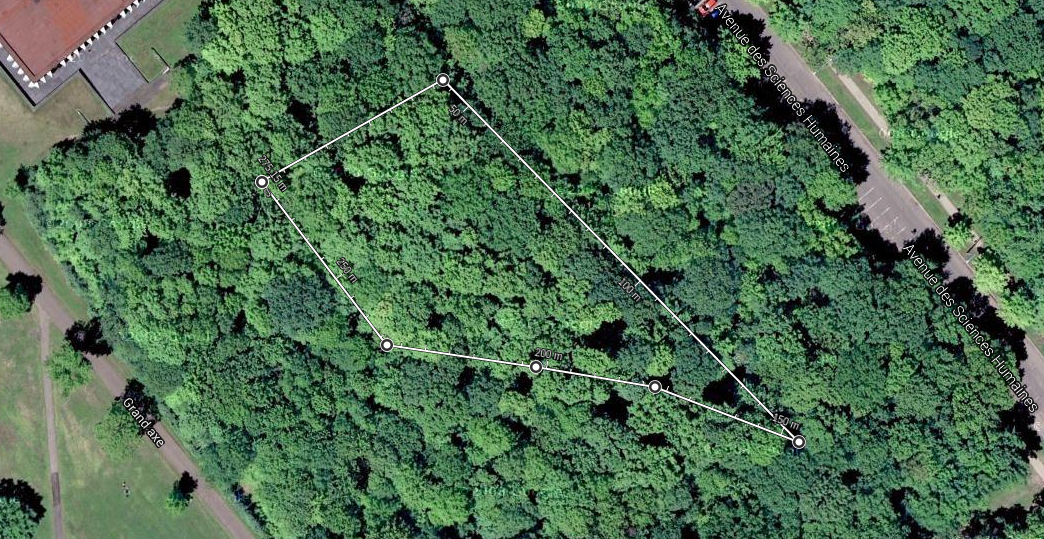
\includegraphics[width=0.455\linewidth]{./figures/path2.png}
            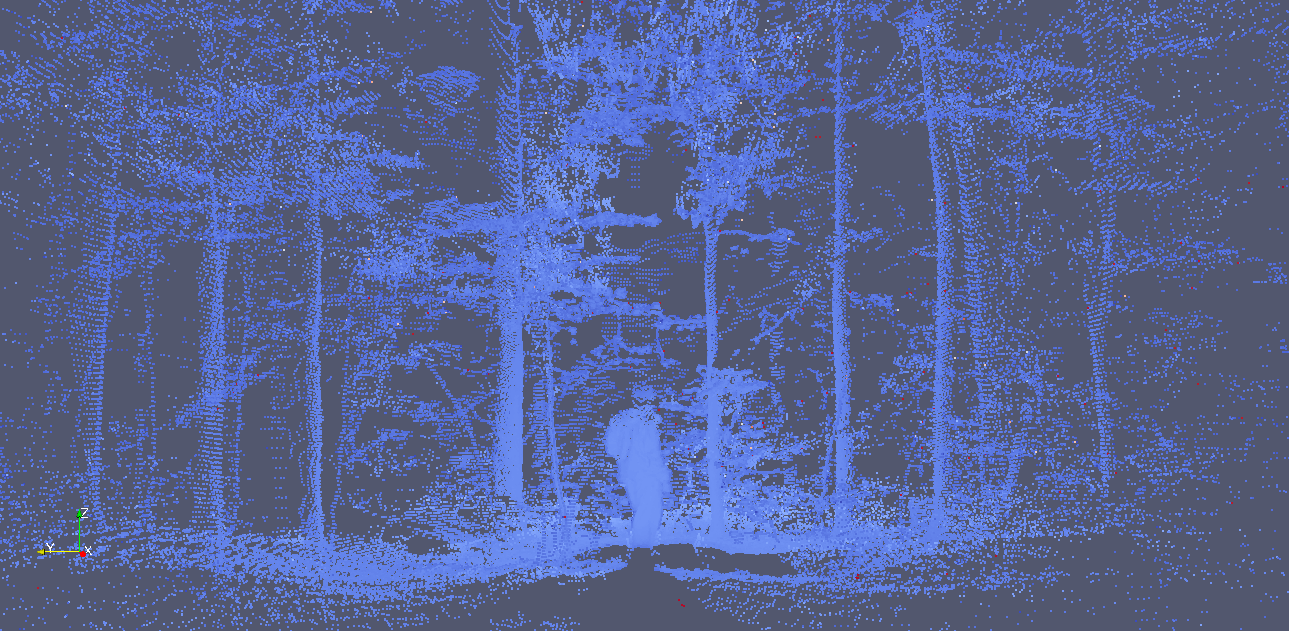
\includegraphics[width=0.48\linewidth]{./figures/sick.png}\\\vspace{-0.8em}
            \begin{flushleft}
                \hspace{1.25em}\tiny Source: Google Maps, (2015)
            \end{flushleft}
        \end{center}

        \textbf{Region of interest}\\
        For localization and mapping in forested environments, tree trunks are generally considered as reliable features ~\cite{Song2012}. To take advantage of this information, it might be desirable to \textbf{limit the region of the 3D data} used to a height that is generally above the low vegetation and obstructions, but below secondary stems and other canopy ~\cite{Mcdaniel2012}. It might increase the robustness against the effect of seasonal changes such as snow coverage and foliage. The figure below shows a potential region of interest that highlight how most trees stand out from other structures.
        \begin{center}
            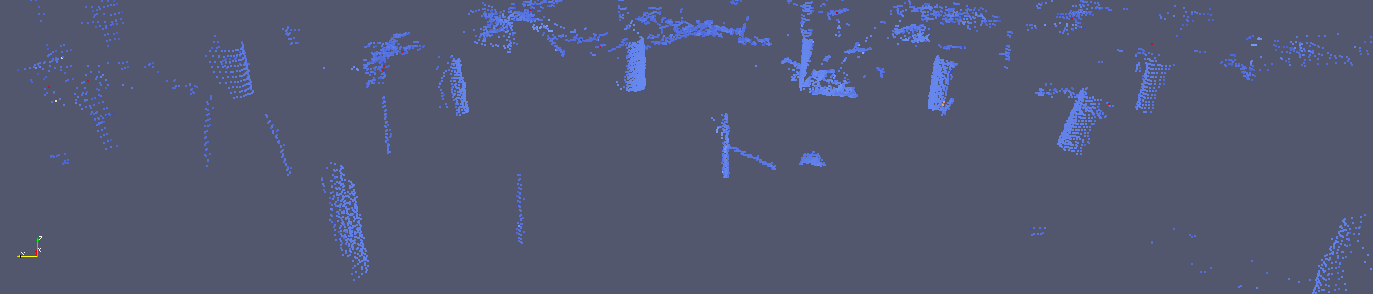
\includegraphics[width=0.95\linewidth]{./figures/pointcloudSlice.png}
        \end{center}

        \textbf{Spatial information for features}\\
        Using BoW removes any spatial dependency between features. Adding low-level spatial information constraint such as feature height might reduce potential mismatch between the input scan and database samples.\vspace{1em}
        % [TODO]: ??? This is similar to geometric constraints employed in many visual SLAM approaches, such as FABMAP.

        \textbf{Data density}\\
        Investigating the relation between data density and scan matching reliability could also lead to a better trade-off between processing time and results quality.\vspace{1em}

        \textbf{Potential 3D features}\\
        There are currently multiple 3D features reported in the literature, for instance:
        % [TODO]: Create a table with this ! - 2015-06-06 04:44pm
        \begin{itemize}
            \item[•] Intrinsic Shape Signatures (ISS) ~\cite{Yu2009};
            \item[•] Normal-Aligned Radial Features (NARF) ~\cite{Steder2011};
            \item[•] Signatures of Histograms of OrienTations (SHOT) ~\cite{Tombari2010};
            \item[•] Fast Point Feature Histogram (FPFH) ~\cite{Rusu2009}.
        \end{itemize}
        Additionally, \textbf{comparative evaluations} ~\cite{Boyer2011} ~\cite{Filipe2014} are also available for a subset of those features, but work is limited to man-made objects and might yield different results in unstructured environments. Also, a \textbf{feature learning} approach could lead to better results for specific environments such as forest.\vspace{1em}

        \textbf{Point cloud based vs range image based features}\\
        Using features based on point cloud instead of range images could benefit from incremental information by merging multiple acquisitions. It might improve results when an environment is seen from a different point of view (trees seen from behind).
    }

\end{poster}

\end{document}
